\section{What waiting buys}\label{to:sec:waiting}

\paragraph{Side information.} Take a memory $M$ whose states all have the same energy, as in an information register, and many copies of a fixed state of $M$ and its quantum side information $O$. Erasing $M$, while leaving $O$ and its correlations with everything else intact, costs $\kB T\ln2\,S(M|O)$ per copy; del Rio et al.\ showed that this much work suffices, even when it is negative~\cite{delRio11}. Without the side information it costs $\kB T\ln2\,S(M)$, more by the mutual information $I(M{:}O)$. When the states of $M$ differ in energy, the reset changes that energy too, and the cost changes with it. A qubit of gap $E$ at $\beta E=\ln2$, in its Gibbs state, is excited with probability $1/3$; resetting it to its ground state costs $\kB T\ln2\,[h_2(1/3)-1/3]=\kB T\ln(3/2)$, that is $0.585$ bits per copy, not the $h_2(1/3)=0.918$ bits of its entropy. This is the rate of a full reset, Theorem~\ref{thm:main-dichotomy}(b) at $p=1$, whose hardest input is this Gibbs state. The law of Section~\ref{to:sec:law} and the integrands below include this energy term. A batch device keeps its outputs as side information until it has cleaned up~\cite[Sec.~7]{FBB21}; a real-time device has already released them. At a fixed input $\rho$, the real-time integrand exceeds the batch one by $m_\rho$, the least such mutual information an implementation must leave, which can be smaller than any particular dilation suggests. For time-covariant channels the optimal batch rate in this thermal-operation model is the thermodynamic capacity $\mathcal T(\Phi)=\max_\rho c_\rho$, where $c_\rho=S(\rho)-S(\Phi(\rho))+\beta\Tr H(\Phi(\rho)-\rho)/\ln2$, so the surcharge between the optimal rates is $\Trt(\Phi)-\mathcal T(\Phi)=\max_\rho(c_\rho+m_\rho)-\max_\rho c_\rho$. It is not an optimum of $m_\rho$ alone, because the two maxima can sit at different inputs. The extra term $m_\rho$ is a correlation cost, input by input; the surcharge compares two optimized totals. For amplitude damping at $p=1/2$ and $\beta E=\ln2$ (Figure~\ref{to:fig:surcharge}), $m_\rho=0.918$ bits at the real-time optimum, while the surcharge is $0.585E-0.154E=0.431E$ per use, that is $0.431$ bits. For a general channel with a returned clock the batch endpoint is instead $B(\Phi)$ of Section~\ref{to:sec:clock}, and the saving from waiting is $\kB T\ln2\,\Trt(\Phi)-B(\Phi)$. The capacity gap remains a benchmark, but it need not be a saving available under that return contract: $X$-dephasing costs $E/2$ per use in both schedules, above its capacity. On inputs diagonal in its basis, a classical channel can leave behind nothing correlated with the outputs it releases, by hiding its randomness in a nearly flat register; coherent inputs can leave a correlation, but they cannot raise the optimized cost (Appendix~\ref{app:channels}). So a classical channel pays nothing extra, much as an information ratchet avoids modularity dissipation by designing internal states that capture the global correlations~\cite{BMC18}; a quantum channel such as partial reset of a qubit must leave its output correlated with what remains, and pays a surcharge at every temperature (Appendix~\ref{app:channels}). Only quantum channels save work by waiting. Here a channel means repeated uses of one memoryless map: classical tasks with several steps can also save work by waiting, as Proposition~\ref{to:prop:rank} shows exactly. This concerns the channel, not the memory: for classical strategies with stochastic outputs, a quantum memory can lower the online cost below that of every classical agent whose memory is a function of the past~\cite{Thompson25}, and only when two causal states form a causally wasteful pair~\cite[Result~2]{Thompson25}.

\begin{figure}[t]
\centering
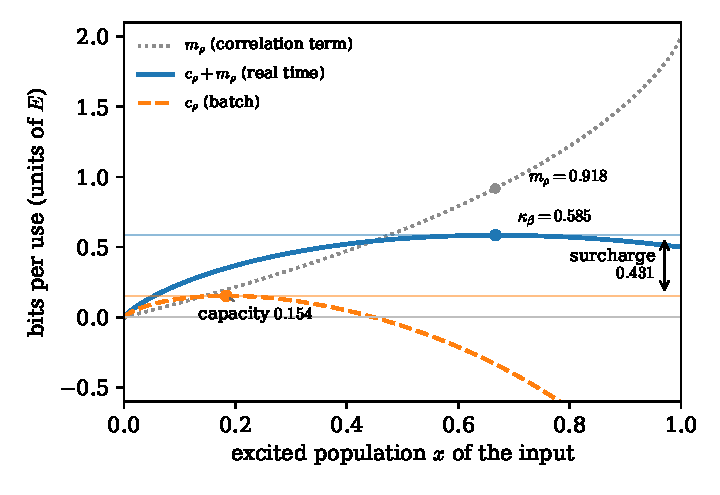
\includegraphics[width=0.62\linewidth]{fig-surcharge.pdf}
\caption{The surcharge is a difference of two maxima. Amplitude damping with $p=1/2$ at $\beta E=\ln2$, so that one bit costs $E$; inputs diagonal in the energy basis, with excited population $x$, attain both maxima. Dashed: the batch integrand $c_\rho=h(x)-h(x/2)-x/2$, whose maximum is the capacity, $0.154$, at $x\approx0.18$. Solid: the real-time integrand $c_\rho+m_\rho=h(x/2)-x/2$, whose maximum is $\Trt=0.585$, at $x=2/3$. Dotted: the correlation term $m_\rho=2h(x/2)-h(x)$. The surcharge, $0.431$, is neither $m_\rho$ at the real-time optimum, $0.918$, nor $m_\rho$ at the batch optimum, $0.197$.}
\label{to:fig:surcharge}
\end{figure}

\paragraph{Error.} For extreme channels, the batch saving requires nonzero error, even when that error vanishes with the block size.

\begin{proposition}[Zero error removes the saving for extreme channels (Appendix~\ref{app:channels})]\label{to:prop:extreme}
If a channel is extreme in the convex set of channels, every implementation with zero error, in batch or in real time, draws free energy from its battery and controller at no less than the real-time rate.
\end{proposition}

Extremality makes the branches of any exact implementation orthogonal~\cite{Choi75}, so the device's entropy rises by exactly the entropy of the complementary output on every input. For amplitude damping at $p=1/2$ and $\beta E=\ln2$, the real-time rate is $0.585\,E$ per use and the batch capacity $0.154\,E$ (Appendix~\ref{app:channels}); the difference is available only to a device that tolerates some error.

\paragraph{Delay.} Let each output be released $b$ steps later than in real time. For independent delayed-choice episodes, in which a qubit is released and the question it must answer arrives $\ell_i$ steps later, the number of episodes that still require an early commitment is $\#\{i:\ell_i>b\}$, and under one-way communication from the party that answers, the entanglement cost is exactly this number (a question that arrives in the same step as the delayed release is taken to arrive first): each such episode is charged one ebit by the monogamy argument of Section~\ref{to:sec:beyond}, and every other episode is answered before its release at no cost. One more step of delay saves $\#\{i:\ell_i=b+1\}$: a step of delay is worth exactly the questions it moves to the accessible side of a release, and has no fixed exchange value. Under the strict real-time rule, where the next input arrives only after the last output has left, waiting longer does not move any question and buys nothing. For repeated uses of one channel, running blocks in batch, with the exponentially small block error that the construction of Faist, Berta and Brand\~ao has at a fixed typicality tolerance (proof of Theorem~\ref{sw:thm:werner}), and taking a union bound over blocks comes within any fixed $\delta>0$ of the batch rate once the delay exceeds $C_\delta\log(n/\varepsilon)$; this construction reaches the batch rate itself only with a delay that grows faster than $\log(n/\varepsilon)$, and the exact work--latency profile is open.

\paragraph{Which carriers to hold.} With several carriers in flight, a schedule can let some of them wait for a later input while others leave. For linear tasks the price of such a schedule is a rank, and the best choice of what to hold is a question about codes. For example, let the late output need the two parities $a_1\oplus a_2$ and $a_2\oplus a_3$, so that $F$ has rows $(1,1,0)$ and $(0,1,1)$. Releasing all three bits costs two bits. Holding any one of them still leaves released columns of rank two, so it saves nothing; holding any two leaves a single nonzero column and lowers the cost to one bit; holding all three makes it zero. A held bit helps only when it completes a late parity, not merely because it is one more bit of storage.

\begin{proposition}[Release rank]\label{to:prop:rank}
Let $F$ be an $\ell\times k$ binary matrix. A device receives $a\in\mathbb F_2^k$ on $k$ bit carriers with zero Hamiltonian. The carriers in a set $L$ must leave, unchanged, before a fresh $b\in\mathbb F_2^\ell$ arrives on $\ell$ further carriers; those in $R=\{1,\dots,k\}\setminus L$ may be held until then. In the end the device returns every first carrier unchanged and dephased, and the second carriers holding $b\oplus Fa$. Let $D$ be everything the device keeps, initially independent of the inputs, and let $F_L$ be the columns of $F$ in $L$.
\begin{enumerate}[label=(\alph*)]
\item For independent uniform $a$ and $b$, every exact implementation raises the entropy of $D$ by at least $\operatorname{rank}F_L$ bits, so, when its controller, battery and Gibbs reservoirs start independent, it dumps heat at least $[\operatorname{rank}F_L-\Delta S_C-\Delta S_W]\,\kB T\ln2$, with $\Delta S_C$ and $\Delta S_W$ the entropy changes of its controller and battery in bits. An energy-conserving implementation raises the entropy by exactly $\operatorname{rank}F_L$ and dumps heat $(1-q)\operatorname{rank}(F_L)\,\kB T\ln2$, where $q$, the probability that its battery misses its final level, can be made as small as desired.
\item If any $m$ carriers may be held, the least cost is $\operatorname{rank}F-\max\{r:d_r(\mathcal C)\le m\}$ bits, where $\mathcal C$ is the row space of $F$ and $d_r(\mathcal C)$, its $r$-th generalized Hamming weight, is the smallest support of an $r$-dimensional subcode~\cite{Wei91}. Holding $m$ carriers lowers the cost at all exactly when $\mathcal C$ has a nonzero word of weight at most $m$, which is NP-complete to decide~\cite{Vardy97}.
\end{enumerate}
\end{proposition}

Holding every carrier costs nothing, and holding one more carrier helps only when it completes a late parity, one that then depends on held carriers alone: the price $\operatorname{rank}F_L=\operatorname{rank}F-\dim\mathcal C(R)$ counts the independent parities of the released bits that the late output still needs, where $\mathcal C(R)$ is the set of late parities supported on held carriers. By part (b), the price of a schedule is a coding invariant of the task: its generalized Hamming weights, which Wei introduced for the wire-tap channel of type II~\cite{Wei91}. The proof is in Appendix~\ref{to:app:rank}.

% =====================================================================
\section{Returning a clock}\label{to:sec:clock}

A channel that is not time-covariant needs a phase reference. If the reference is finite-dimensional and must come back exactly, and the battery is stationary, no such channel can be run at any work cost: by the no-broadcasting theorem for asymmetry, a bounded reference used to implement an operation that is not covariant is necessarily degraded~\cite{MarvianSpekkens19,LostaglioMuller19}; if it need only come back approximately, every channel runs in real time at the rate $\Trt$ (Appendix~\ref{app:channels}, with the signed battery deviation of Table~\ref{tab:exceptions}). For a gate the reference then pays in other currencies: capital at least of order $n/(\varepsilon+\eta)$, baths whose energy range grows at least like $n/\sqrt\varepsilon$, and an energy that returns only as a lottery (Appendix~\ref{app:batch}). The capital has the scaling of the reference-size laws of Chiribella, Yang and Renner and of Tajima, Shiraishi and Saito~\cite{ChiribellaYangRenner21,TSS20}. Channels that are not gates can need far less: a Gibbs-preserving qubit channel that is not time-covariant runs in batch at zero work with a clock whose spread grows like $\sqrt n$ (Appendix~\ref{app:batch}).

In batch the returned clock has an exact price. Let $\Psi$ be a complementary channel, $D=\Phi^*(H)-H$ and
\[
B(\Phi)=\max\bigl\{\Tr\rho D+\kB T\ln2\,[S(\sigma)-S(\Phi(\sigma))]\;:\;\Psi(\rho)=\Psi(\sigma)\bigr\}.
\]

\begin{theorem}[The batch law with a returned clock (Appendix~\ref{app:batch})]\label{to:thm:batchlaw}
With a battery that starts in an energy eigenstate and a controller that returns approximately, all of it and not only the clock, the optimal batch work per use of every finite channel is $B(\Phi)$, attained with deterministic work. It equals $\kB T\ln2\,\mathcal T(\Phi)$, the thermodynamic capacity in energy units, whenever $D$ lies in the span of the products $A_i^*A_j$ of Kraus operators, and a Gibbs-preserving channel is free exactly when it does.
\end{theorem}

Two inputs can be charged separately, one for energy and one for entropy, exactly when the environment cannot tell them apart. When the environment can carry the energy change, input by input on average, the clock never has to absorb an energy that depends on the input, and the capacity is reached. This makes precise the obstruction that Faist, Berta and Brand\~ao anticipated: for superposed inputs of different energy, the environment must compensate the energy difference without disturbing the process~\cite{FBB19}. A returned clock can supply phase, but it cannot provide net extensive energy: for every observer its actual mean energy change must be sublinear. It can still make large loans that depend on the branch, as long as their mean is refunded. When the environment cannot carry the energy change, the remainder may have to be paid, but it need not be: a unitary gate changes no entropy, so for the Hadamard gate $B(\Phi)$ equals the capacity although $D$ lies outside the span (Section~\ref{sec:channel-statements}). Qubit dephasing in the $X$ basis costs $E/2$ per use in batch, exactly its real-time cost and above its capacity; some Gibbs-preserving channels, of capacity zero, cost work of order $n$; and every Gibbs-preserving qubit channel is free in batch with a returned clock (Appendix~\ref{app:batch}). The span of the products $A_i^*A_j$ is the non-commutative confusability graph of Duan, Severini and Winter~\cite{DSW13}. The same condition separates small clocks from large ones. When $D$ lies outside the span, the channel's orbit under time translation, whose generator is exactly $D$, can be estimated at the Heisenberg limit~\cite{ZhouJiang21}. A code built as in~\cite[Sec.~V]{ZhouJiang21} turns $n$ uses of any reliable implementation into a probe that reads the controller's clock to within $O(1/n)$, so no clock whose spread grows more slowly than $n$ can run it reliably, at any work (Appendix~\ref{app:batch}).

\begin{table}[tbp]
\centering
\small
\begin{tabular}{>{\raggedright\arraybackslash}p{4.6cm}>{\raggedright\arraybackslash}p{6.6cm}l}
\toprule
Schedule and clock & Processes that cost nothing & Decidable\\
\midrule
Batch, Gibbs-preserving maps free~\cite{FBB21} & Gibbs-preserving channels & yes\\
Batch, clock returned & Gibbs-preserving, with $H-\Phi^*H\in\mathrm{span}\{A_i^*A_j\}$ & yes\\
Real time & limits of thermal operations (Appendix~\ref{app:channels}) & no\\
\bottomrule
\end{tabular}
\caption{The free channels shrink as the operational model tightens: Gibbs-preserving maps taken as free operations, thermal operations with a returned clock in batch, and thermal operations in real time. Each inclusion is strict: a Gibbs-preserving qutrit separates the first two rows (Appendix~\ref{app:batch}), the Werner--Holevo channel, which is not factorizable~\cite{HaagerupMusat11}, the last two. Decidability is for exact algebraic data, under the hypothesis of Theorem~\ref{thm:main-undecidable}.}\label{to:tab:ladder}
\end{table}

\paragraph{A process and its time reverse.} For a Gibbs-preserving channel, the reverse process of quantum fluctuation theorems~\cite{Crooks08,KwonKim19} is its Petz map $\Phi^\sharp(\sigma)=\gamma^{1/2}\Phi^*(\gamma^{-1/2}\sigma\gamma^{-1/2})\gamma^{1/2}$. Thermal operations are closed under this reversal. With a returned clock, the criterion of Theorem~\ref{to:thm:batchlaw} is not: on a qutrit there is a Gibbs-preserving channel that costs $0.1547\,\kB T$ per use while its reverse costs nothing (Appendix~\ref{app:batch}). Which direction is free is decided by two linear tests on the Kraus operators. The asymmetry is not generic: channels of full Kraus rank pass both tests, so any fixed amount of full-rank thermal noise removes it, and separated pairs lie on the boundary of the set of Gibbs-preserving channels, as Tajima and Takagi found for Gibbs-preserving maps whose coherence cost diverges~\cite[Suppl.\ Prop.~S.11]{TajimaTakagi25}. For a finite device the threshold is set by the horizon: noise removes the asymmetry only when the expected number of noisy uses grows without bound, so noise per use small compared with the inverse of the number of uses leaves the full cost in place (Appendix~\ref{app:batch}). In coherence the same pair is already asymmetric, as Tajima and Takagi found for detecting versus creating coherence~\cite{TajimaTakagi25}: by their theorem the forward channel, which keeps a pair of orthogonal coherent inputs perfectly distinguishable, needs coherence that diverges as the error vanishes, while its reverse, which reads energy populations and prepares coherent states, can be implemented with finite coherence by the construction they give for maps of that kind~\cite[Suppl.\ Sec.~IV]{TajimaTakagi25}. With a returned clock the asymmetry appears in work. It is an implementation asymmetry created by the obligation to return the clock. It does not violate any fluctuation theorem, and it is not carried by the clock, whose entropy changes by $o(n)$.

% =====================================================================
